\documentclass{article}
\usepackage[utf8]{inputenc}
\usepackage[margin=1in]{geometry}
\usepackage{amsmath}
\usepackage{graphicx}
\graphicspath{{frames/}}
\setlength{\parindent}{0em}
\setlength{\parskip}{0.5em}

\title{CTA200 Project}
\author{Emily Crawley}
\date{14/05/2021}

\begin{document}

\maketitle

\section*{Reading GADGET-2 files}
The snapshots used in this project are of the GADGET-2 Format 1, which is a legacy format, but has extensive documentation as to its format. The snapshot files are binary files with a 256-byte header, followed by particle positions, velocities, and all other required info. It is important to note that both before and after each block there is a uint32 value designating the size of the block in bytes.

That is, the snapshot files are structured like:


HEADER SIZE (4 bytes)

HEADER (256 bytes)

HEADER SIZE (4 bytes)

BLOCK 1 SIZE (4 bytes)

BLOCK 1 (sizeof(float)*\{BLOCK 1 SIZE\} bytes)

BLOCK 1 SIZE (4 bytes)

...

The comprehensive layout of these legacy Format 1 files as well as the other formats including HDF5 can be found in the official documentation.

The header includes the separate numbers of each of the six types of particle in a given simulation. These are always in the same order and appear in that order in the positions and velocities blocks as well: \texttt{gas, halo, disk, bulge, star, bndry}.

I wrote a C function to read in the particle positions but didn't quite have time to figure out getting the C code into Python, so I translated it to Python. The function currently only reads in particle positions but reading in any other needed data follows the same idea. I originally used the package \texttt{pynbody} to read the snapshot files and to test out some of the snapshots with the Amiga Halo Finder but ran into some issues with missing gravitational softening length - but this package has extensive functionality for working alongside AHF.

\section*{Visualizing the simulations}
GADGET-2 includes by default a few different initial conditions files. I generated some short simulations using the \texttt{galaxy} and \texttt{cluster} examples. The exported animations can be found in the videos folder, or run again using the command format \texttt{visualize cluster 3d}.

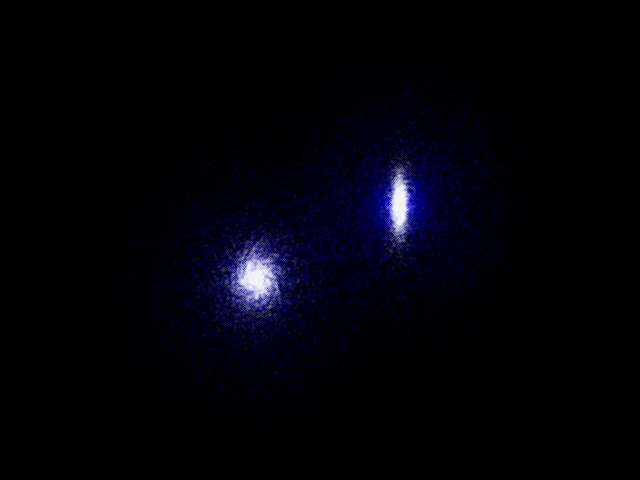
\includegraphics[scale=0.4]{frame6}
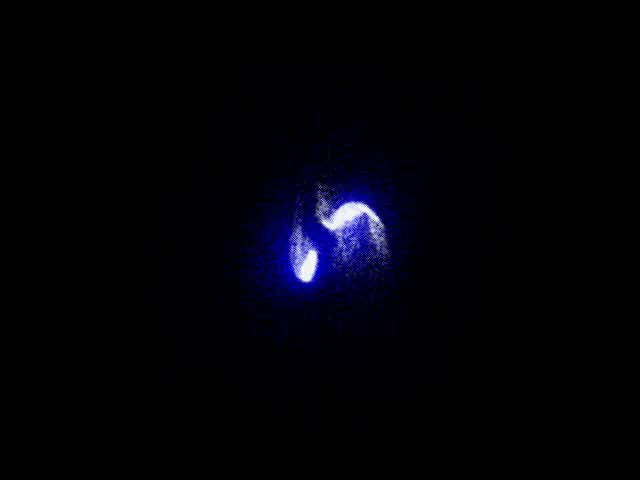
\includegraphics[scale=0.4]{frame11}
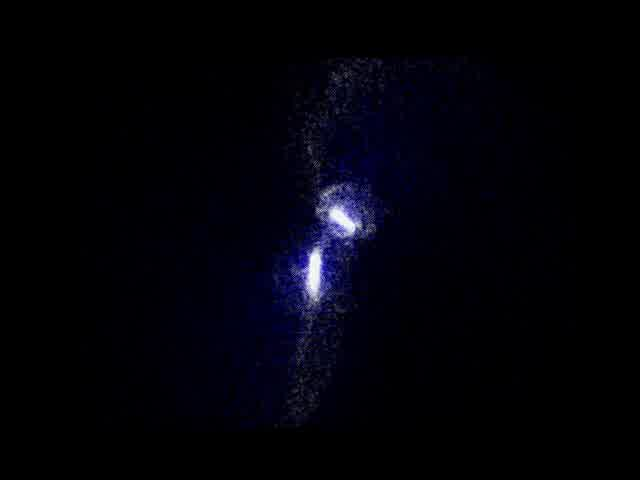
\includegraphics[scale=0.4]{frame17}
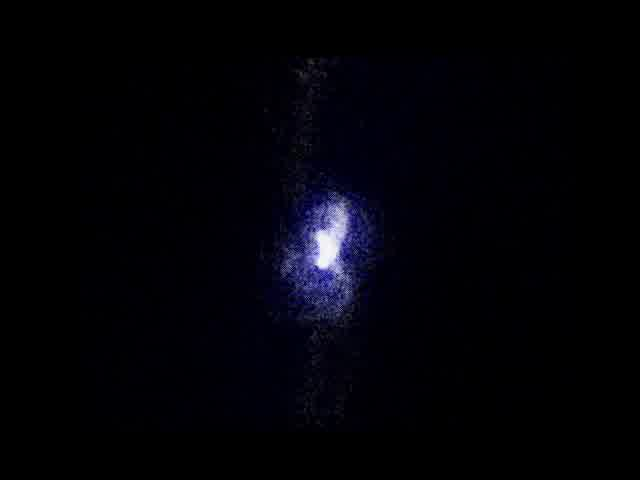
\includegraphics[scale=0.4]{frame21}

\end{document}